\documentclass[a4paper]{article} 
\usepackage[backend=biber]{biblatex}
\usepackage{float}
\usepackage{graphicx}
\addbibresource{ref.bib}
\addtolength{\hoffset}{-2.25cm}
\addtolength{\textwidth}{4.5cm}
\addtolength{\voffset}{-3.25cm}
\addtolength{\textheight}{5cm}
\setlength{\parskip}{0pt}
\setlength{\parindent}{0in}

%----------------------------------------------------------------------------------------
%	PACKAGES AND OTHER DOCUMENT CONFIGURATIONS
%----------------------------------------------------------------------------------------

\usepackage{blindtext} % Package to generate dummy text
\usepackage{charter} % Use the Charter font
\usepackage[utf8]{inputenc} % Use UTF-8 encoding
\usepackage{microtype} % Slightly tweak font spacing for aesthetics
\usepackage[english]{babel} % Language hyphenation and typographical rules
\usepackage{amsthm, amsmath, amssymb} % Mathematical typesetting
\usepackage{float} % Improved interface for floating objects
\usepackage[final, colorlinks = true, 
            linkcolor = black, 
            citecolor = black]{hyperref} % For hyperlinks in the PDF
\usepackage{graphicx, multicol} % Enhanced support for graphics
\usepackage{xcolor} % Driver-independent color extensions
\usepackage{marvosym, wasysym} % More symbols
\usepackage{rotating} % Rotation tools
\usepackage{censor} % Facilities for controlling restricted text
\usepackage{booktabs} % Enhances quality of tables
\usepackage{csquotes} % Context sensitive quotation facilities
\usepackage[nodayofweek]{datetime} % Uses YEAR-MONTH-DAY format for dates
\renewcommand{\dateseparator}{-} % Sets dateseparator to '-'
\usepackage{fancyhdr} % Headers and footers
\pagestyle{fancy} % All pages have headers and footers
\fancyhead{}\renewcommand{\headrulewidth}{0pt} % Blank out the default header
\fancyfoot[L]{} % Custom footer text
\fancyfoot[C]{} % Custom footer text
\fancyfoot[R]{\thepage} % Custom footer text
\newcommand{\note}[1]{\marginpar{\scriptsize \textcolor{red}{#1}}} % Enables comments in red on margin

%----------------------------------------------------------------------------------------

\begin{document}

%-------------------------------
%	TITLE SECTION
%-------------------------------

\fancyhead[C]{}
\hrule \medskip % Upper rule
\begin{minipage}{0.295\textwidth} 
\raggedright
\footnotesize
Project Report\hfill\\   
Group-5\hfill\\
CSE333,Monsoon 2020
\end{minipage}
\begin{minipage}{0.4\textwidth} 
\centering 
\large 
OpenGL based Real Time Ray Tracer\\ 
\normalsize 
Aditya Singh Rathore (2018007)\\
Gaurav Rai (PhD) 
\end{minipage}
\begin{minipage}{0.295\textwidth} 
\raggedleft
\today\hfill\\
\end{minipage}
\medskip\hrule 
\bigskip
%-------------------------------
%	CONTENTS
%-------------------------------
\begin{abstract}
    In this project we aim to implement an OpenGL based Ray tracer. We create a 
    full screen quad and use the fragment shader to compute color of each pixel.
    Using the pixel coordinates, we compute rays and find intersection with two 
    primitives-Sphere and Square. Further, we implement Blinn-Phong shading, shadows
    and reflection effects. 
\end{abstract}

\section{Literature Review}

Ray tracing is a simple and elegant technique. We found all information needed 
for implementing ray fracer in Chapter 4 and 13 of Peter Shirley's Book 
Fundamentals of computer Graphics.\cite{shirley} which describes a recursive ray
tracer. We have built our program on the algorithm as descibed in above book.

\vspace{\baselineskip} 

Further, to test Realtime nature of the scene, we have used a camera for demonstration.
General idea in all camera movement is to capture keyboard and mouse displacement 
in every frame and compare with previous frame position, thus infering it as movement of 
object. We used idea described in this website : \url{http://www.opengl-tutorial.org/beginners-tutorials/tutorial-6-keyboard-and-mouse/}

\vspace{\baselineskip}

For intersection of ray with primitives - Square and Sphere, we found material in 
Peter Shirley's book to be quite sufficient. The general idea is to try and find 
point of intersection with primitive and ray. This would be solved to find the 
parameter $t$. if $t>0$, we might have an intersection. Stack Overflow discussion
\url{https://computergraphics.stackexchange.com/questions/8418/get-intersection-ray-with-square}
provides a good method for any arbitrary oriented square.   

\section{Approach}

\subsection{Ray Generation}
\begin{itemize}
    \item We created a full screen quad.
    \item We know that Fragment shader will be called on each pixel.
    \item In the fragment shader, we can get the coordinates of each pixel.
    \item We pass camera position and direction as uniform to the shader.
    \item Using camera details and pixel coordinates, we can generate parameterised equation of ray $e + td$.
    $e$ is origin of ray, $d$ is the direction and parameter $t$. 
\end{itemize}
 
\subsection{Camera}

\subsubsection{Change in orientation}
\begin{itemize}
    \item We use change in $(u,v)$ coordinated of mouse with respect to centre point of screen.
    \item Change in $u$ coordinate is change in orientation along $Horizontal$ $Angle$.
    \item Change in $u$ coordinate is change in orientation along $Vertical$ $Angle$.
\end{itemize}

\subsubsection{Change in Position}
\begin{itemize}
    \item We keep tract of arrow keys placed, per frame. 
    \item We define a fixed displacement in the direction camera is looking at every time key is pressed.
    \item This is the shift in position of camera. 
\end{itemize}
\subsection{Object Creation}
\begin{itemize}
    \item Each primitive is represented in 3D space. Square using 4 points and sphere using centre and radius.
    \item We solve $e+td$ and primitive to find the parameter $t$. 
    \item If $t > 0$, we have a point of intersection.
    \item For every intersection, we color the pixel with the color of object.
    \item If there is no intersection, there is no object. We color this pixel with background color.
\end{itemize}

\subsection{Blinn Phong shading and shadows}
\begin{itemize}
    \item Once we find a valid intersection, we calculate and store its normal.
    \item Point of intersection can be calculated using the value of parameter $t$.
    \item We then use Blinn-Phong shading model for each light source.
    \item For every light source, we check if a ray originating at point of intersection 
    and going towards a light source intersects any other object. 
    \item If it does, that point will not get light, it will be in shadow of the object it 
    intersects. 
\end{itemize}

\subsection{Reflection}
\begin{itemize}
    \item If the ray intersects a reflective surface, we note this fact.
    \item From the surface, we generate the reflected ray with ray direction and surface normal.
    \item We find the point where this reflected ray intersects. That point's color is the color 
    of this point (as it will reflect this color towards eye ($-ray\_direction$)).
    \item However, too many rays can get created in the process. Thus, we limit it to a 
    certain maximum number of reflections.
\end{itemize}

\bigskip

\section{Milestones}
\subsection{Completed}
\begin{itemize}
    \item Ray Generation
    \item Object Creation
    \item Ray-Object Intersection
    \item Blinn Phong shading and shadows 
    \item Dielectrics : Reflection 
\end{itemize}

\subsection{Could not be achieved}
\begin{itemize}
    \item \item Dielectrics : Refraction
\end{itemize}

\bigskip

\section{Implementation Details}

\subsection{Camera}

\bigskip

\section{Outcomes}

\subsection{Object Creation}
\begin{itemize}
    \item We are able to achieve object creation of primitive and complex structures
    from combining primitives.

    \item Our intersection algorithm work in all orientations of objects.    
\end{itemize}

\subsection{Camera}
\begin{itemize}
    \item Camera movement is smooth and accurate.
    \item However, it keeps mouse occupied, thus, complicating any UI gadgets usage.
\end{itemize}

\subsection{Blinn-Phong Shading}
\begin{itemize}
    \item We get good results with no distortions, even with multiple light sources.
    \item Shadows are accurate. 
    \item Well modelled parametrs can produce results indistinguishible from reality.
\end{itemize}

\subsection{Dielectrics}
\begin{itemize}
    
    \item Multiple reflections are handled well. However, at scenarios when number of reflections is 
    beyond the $Max\_depth$, we get dark spot.

    \item Performance is hindered significantly when number of reflective objects are increased. 

    \item With 3 adjacent mirrors and 2 spherical mirrors placed infront of each other, we get good frame rates of around $125$ $fps$. 

\end{itemize}

\subsection{Screenshots}

\begin{figure}[H]
    \centering
    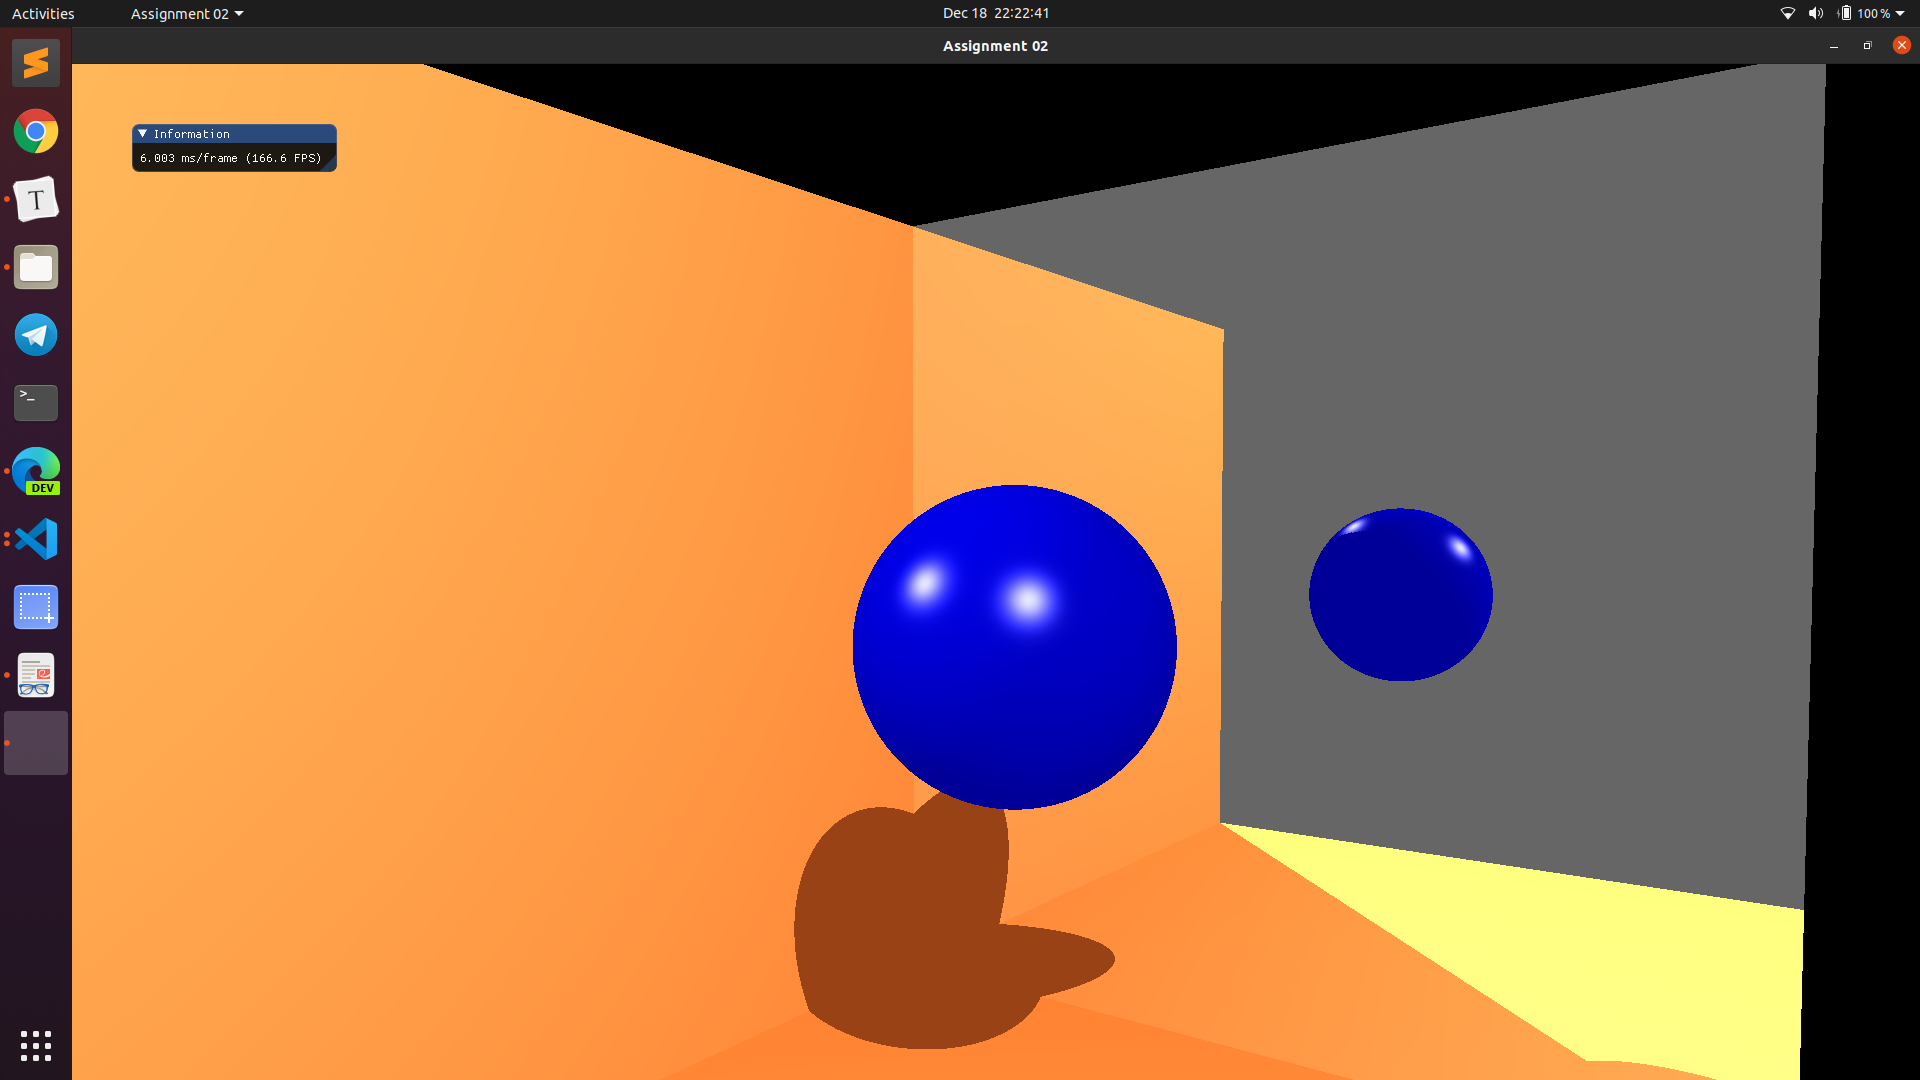
\includegraphics[width=1.0\textwidth]{Images/OneMirror.png}
    \caption{A simple reflection with square mirror.}
\end{figure}

\begin{figure}[H]
    \centering
    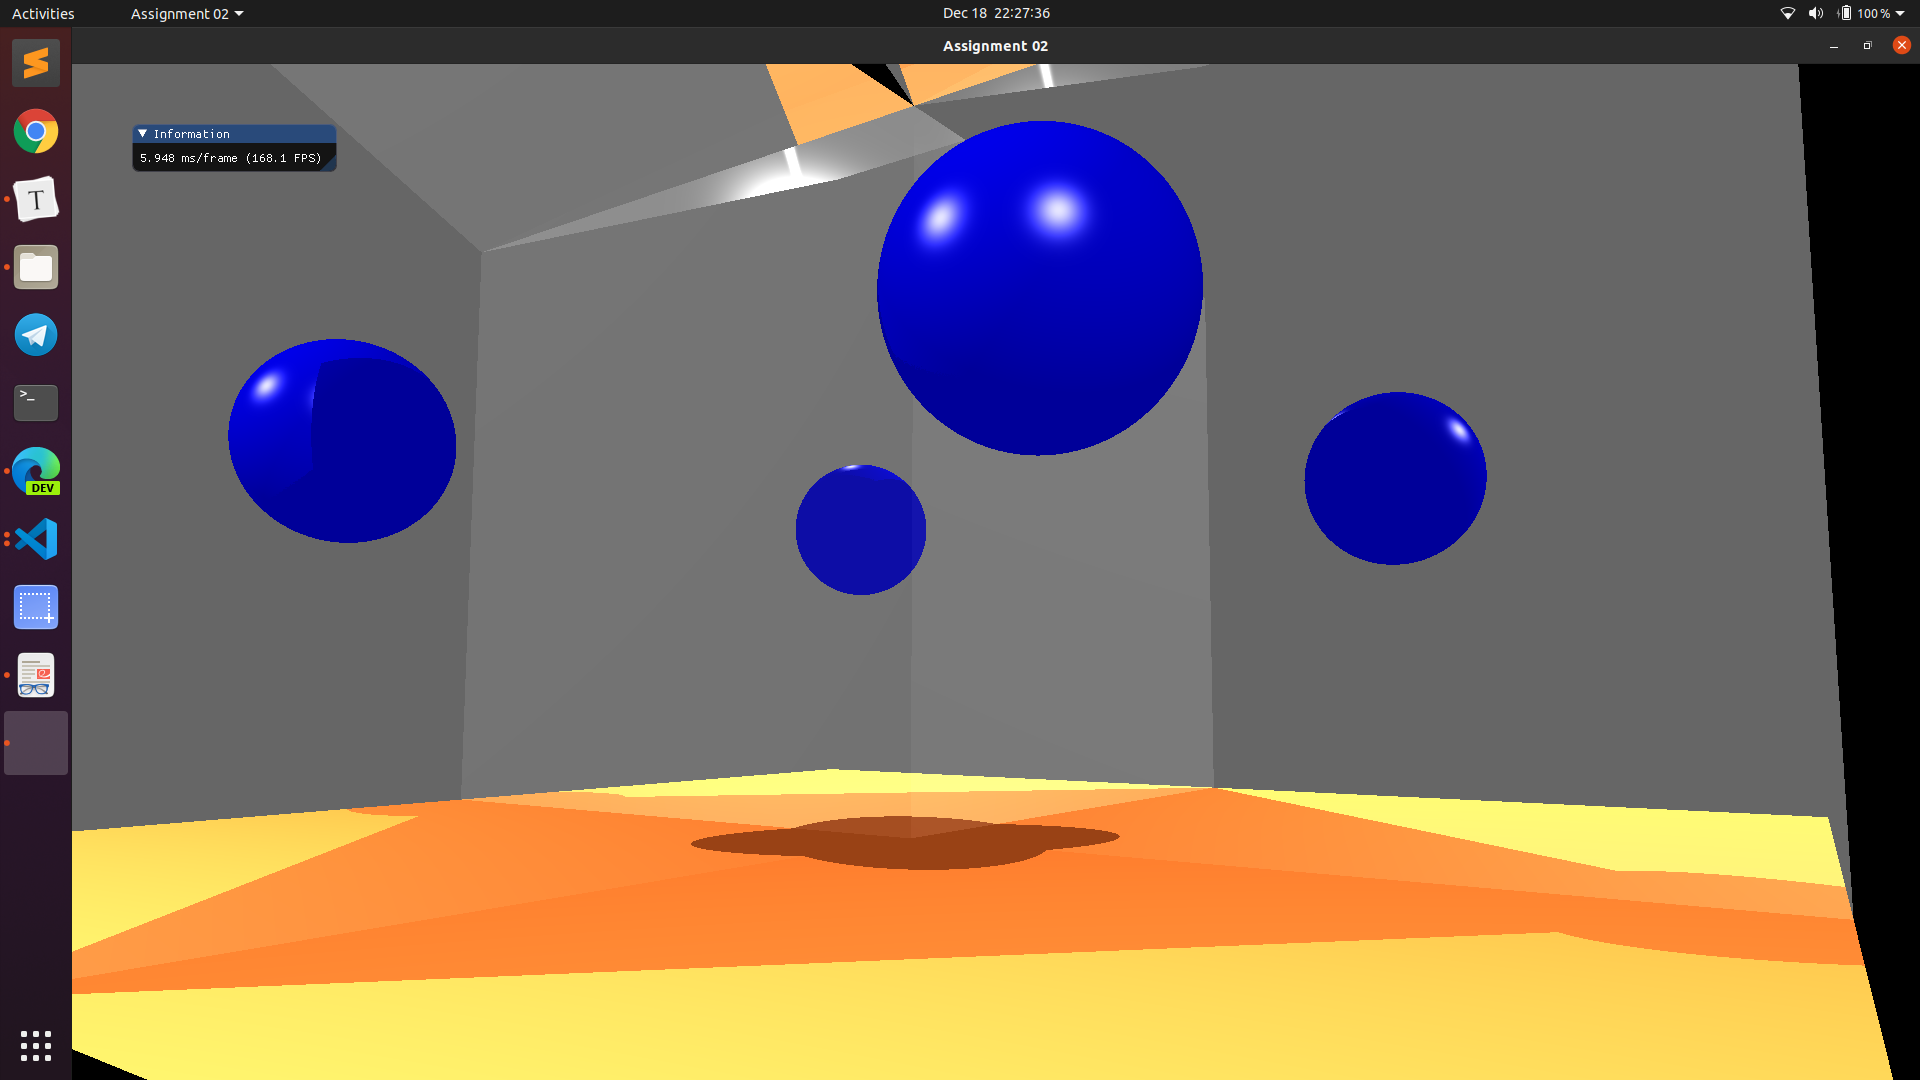
\includegraphics[width=1.0\textwidth]{Images/MultipleReflections.png}
    \caption{Single Object With multiple reflective surfaces.}
\end{figure}

\begin{figure}[H]
    \centering
    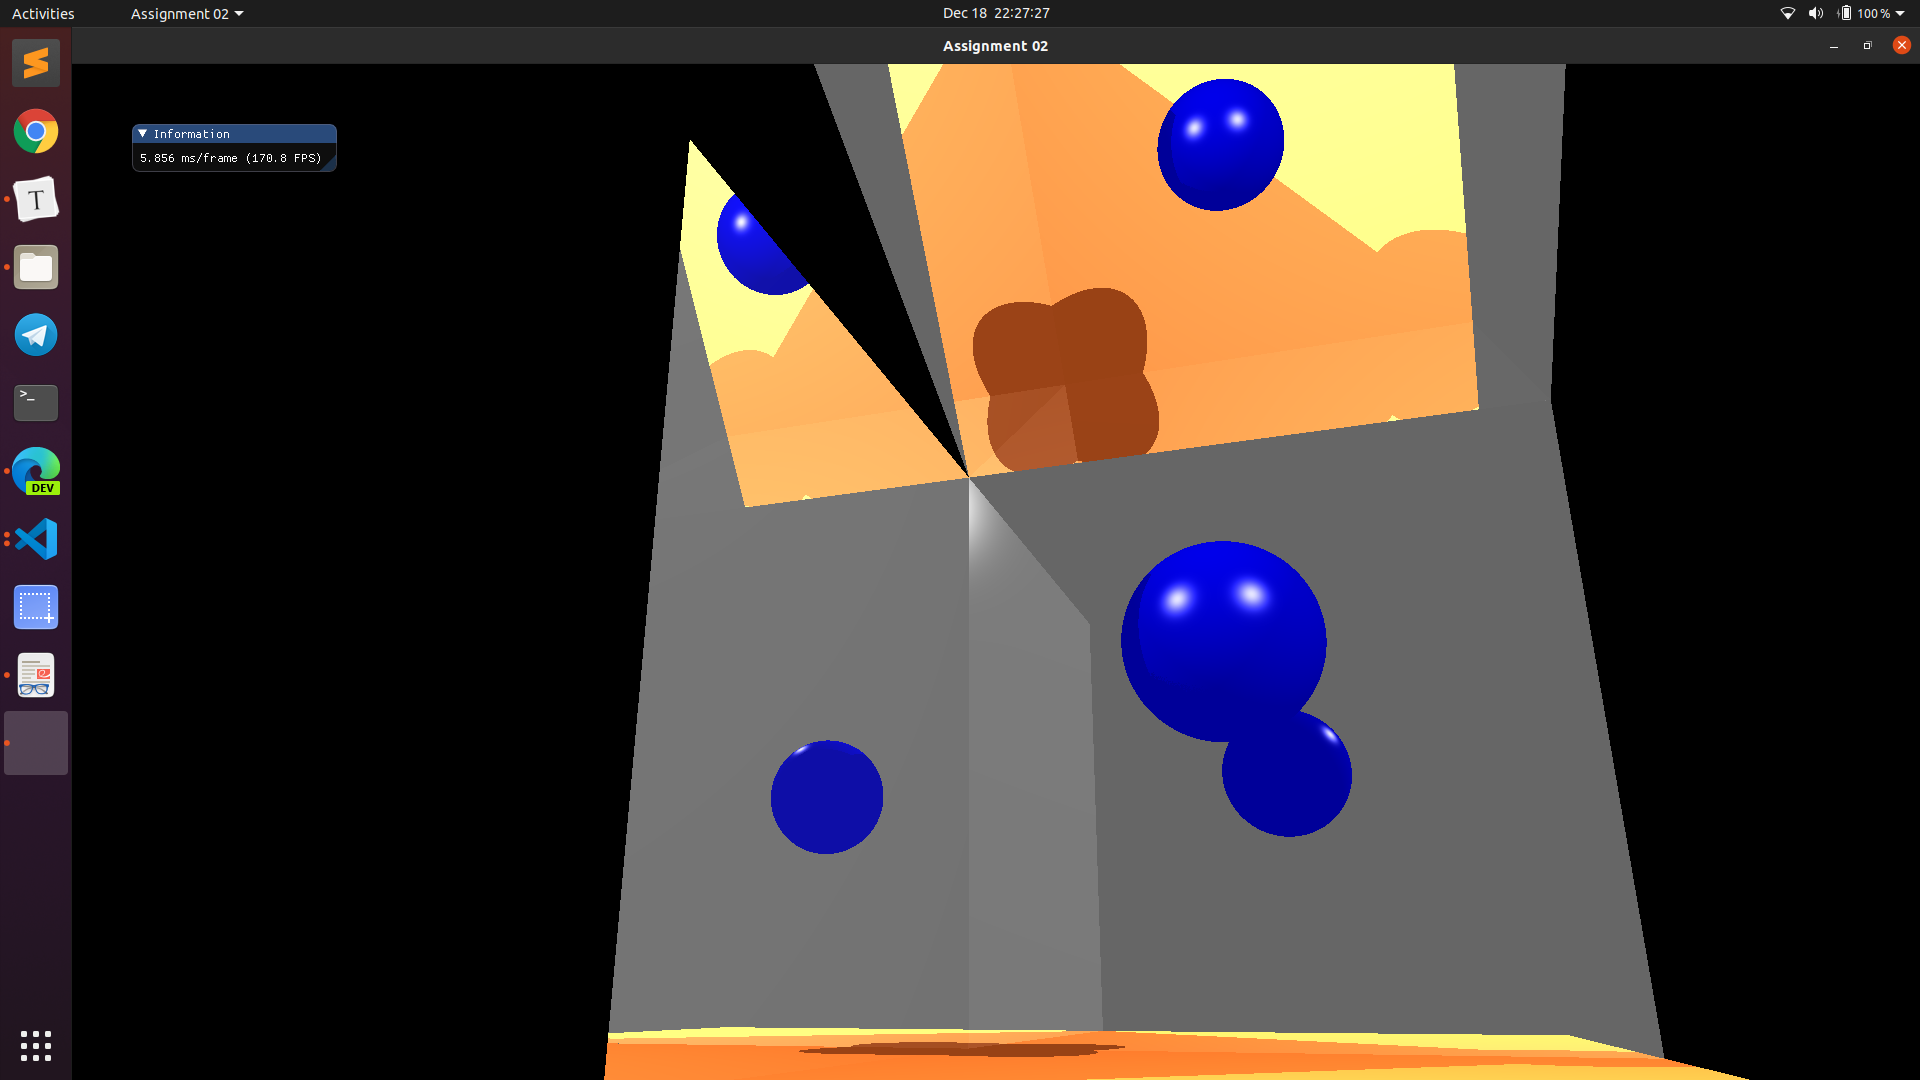
\includegraphics[width=1.0\textwidth]{Images/NonAxisAllignedMirror.png}
    \caption{Non Axis Alligned Square mirror.}
\end{figure}

\begin{figure}[H]
    \centering
    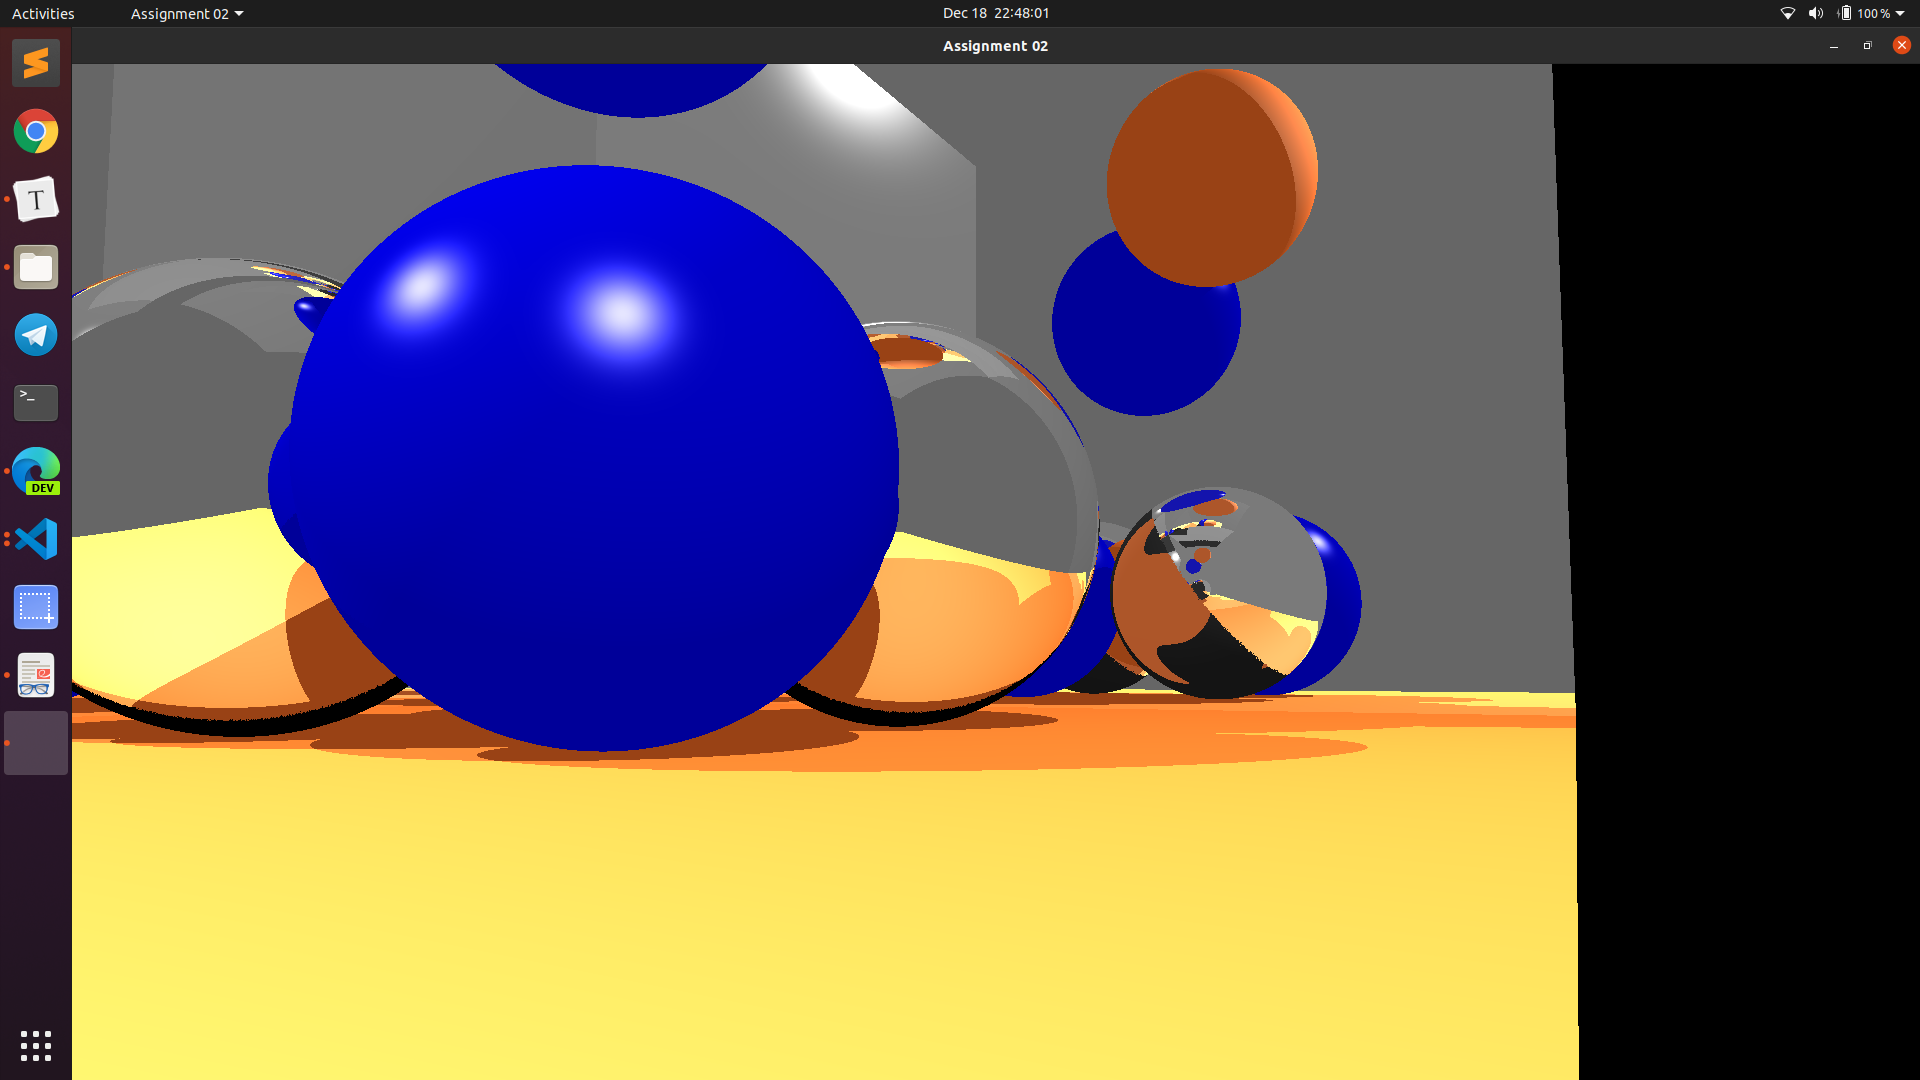
\includegraphics[width=0.8\textwidth]{Images/CloseUp.png}
    \caption{Spherical Mirrors.}
\end{figure}

\begin{figure}[H]
    \centering
    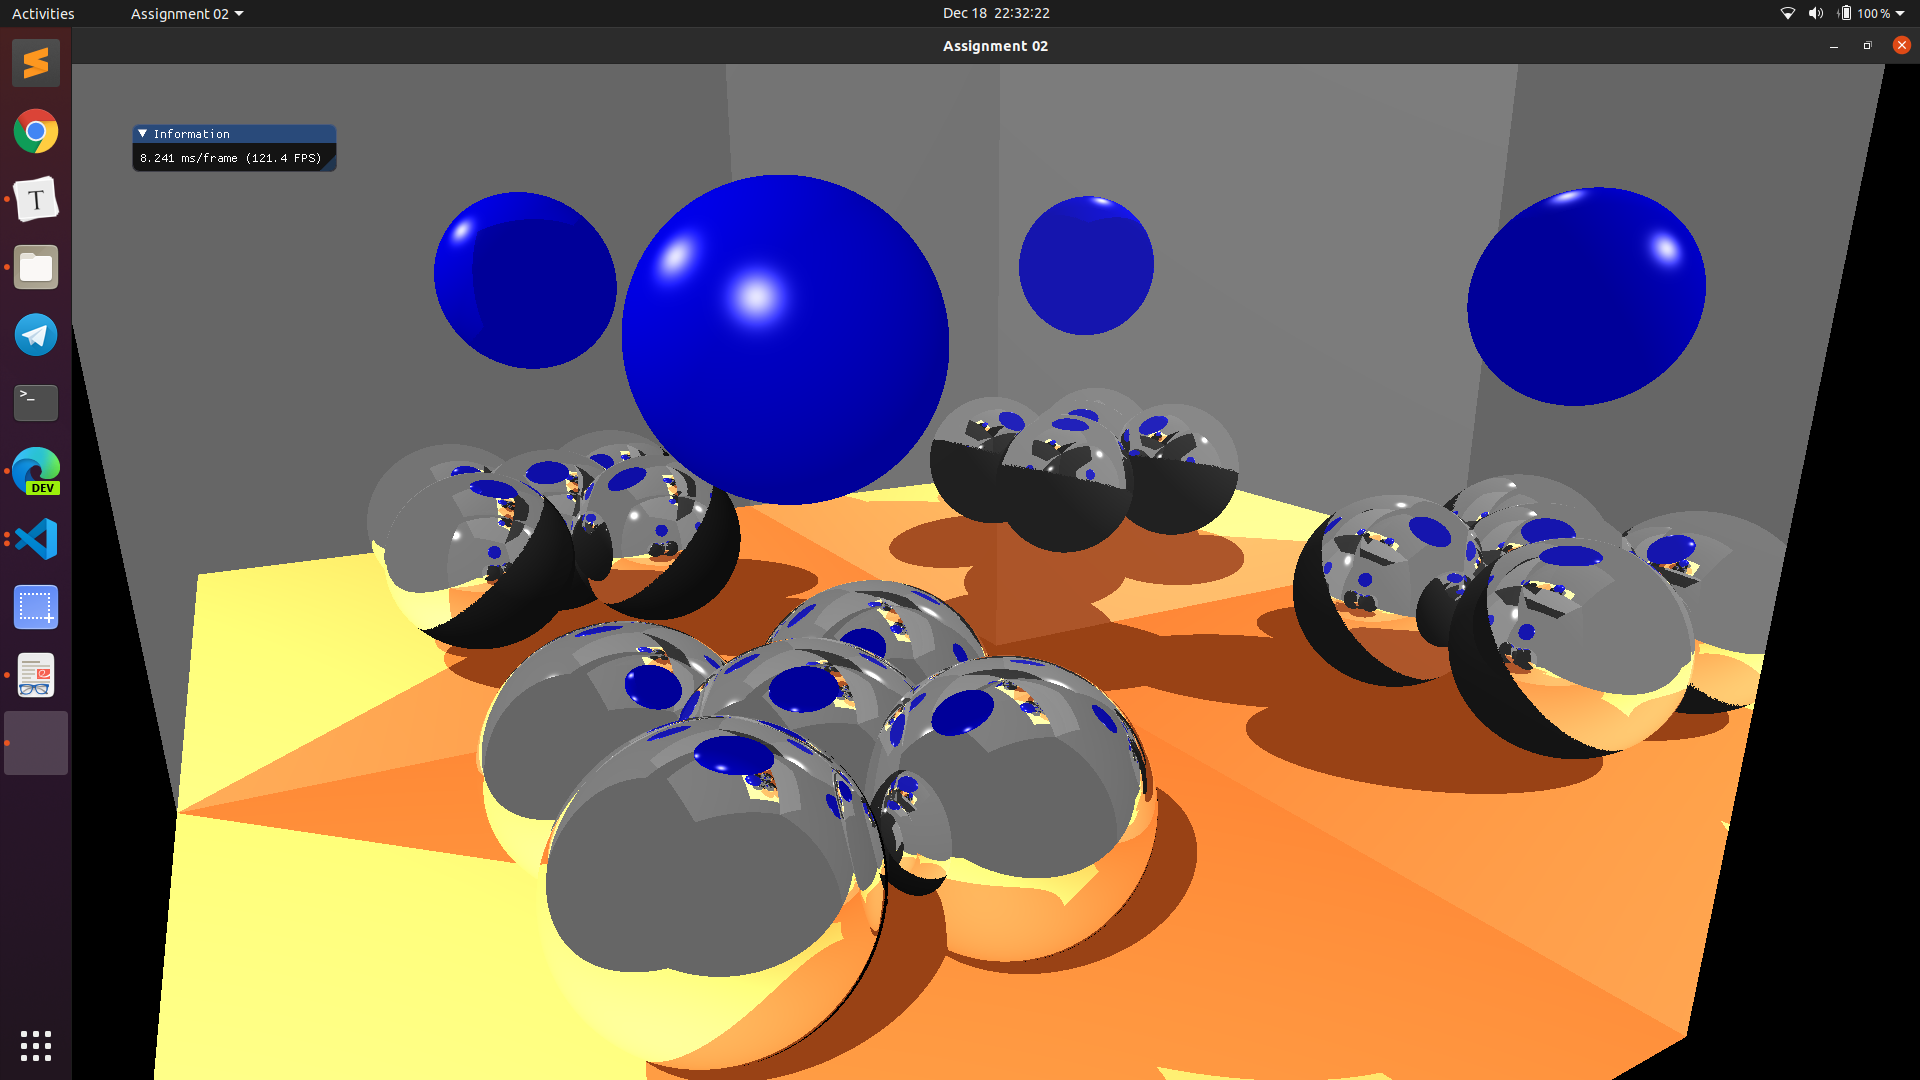
\includegraphics[width=0.8\textwidth]{Images/LimitsOfMultipleReflection.png}
    \caption{Multiple Reflections from multiple surfaces. Note sphereical surfaces have dark spots when reflections exceed maximum depth.}
\end{figure}

\begin{figure}[H]
    \centering
    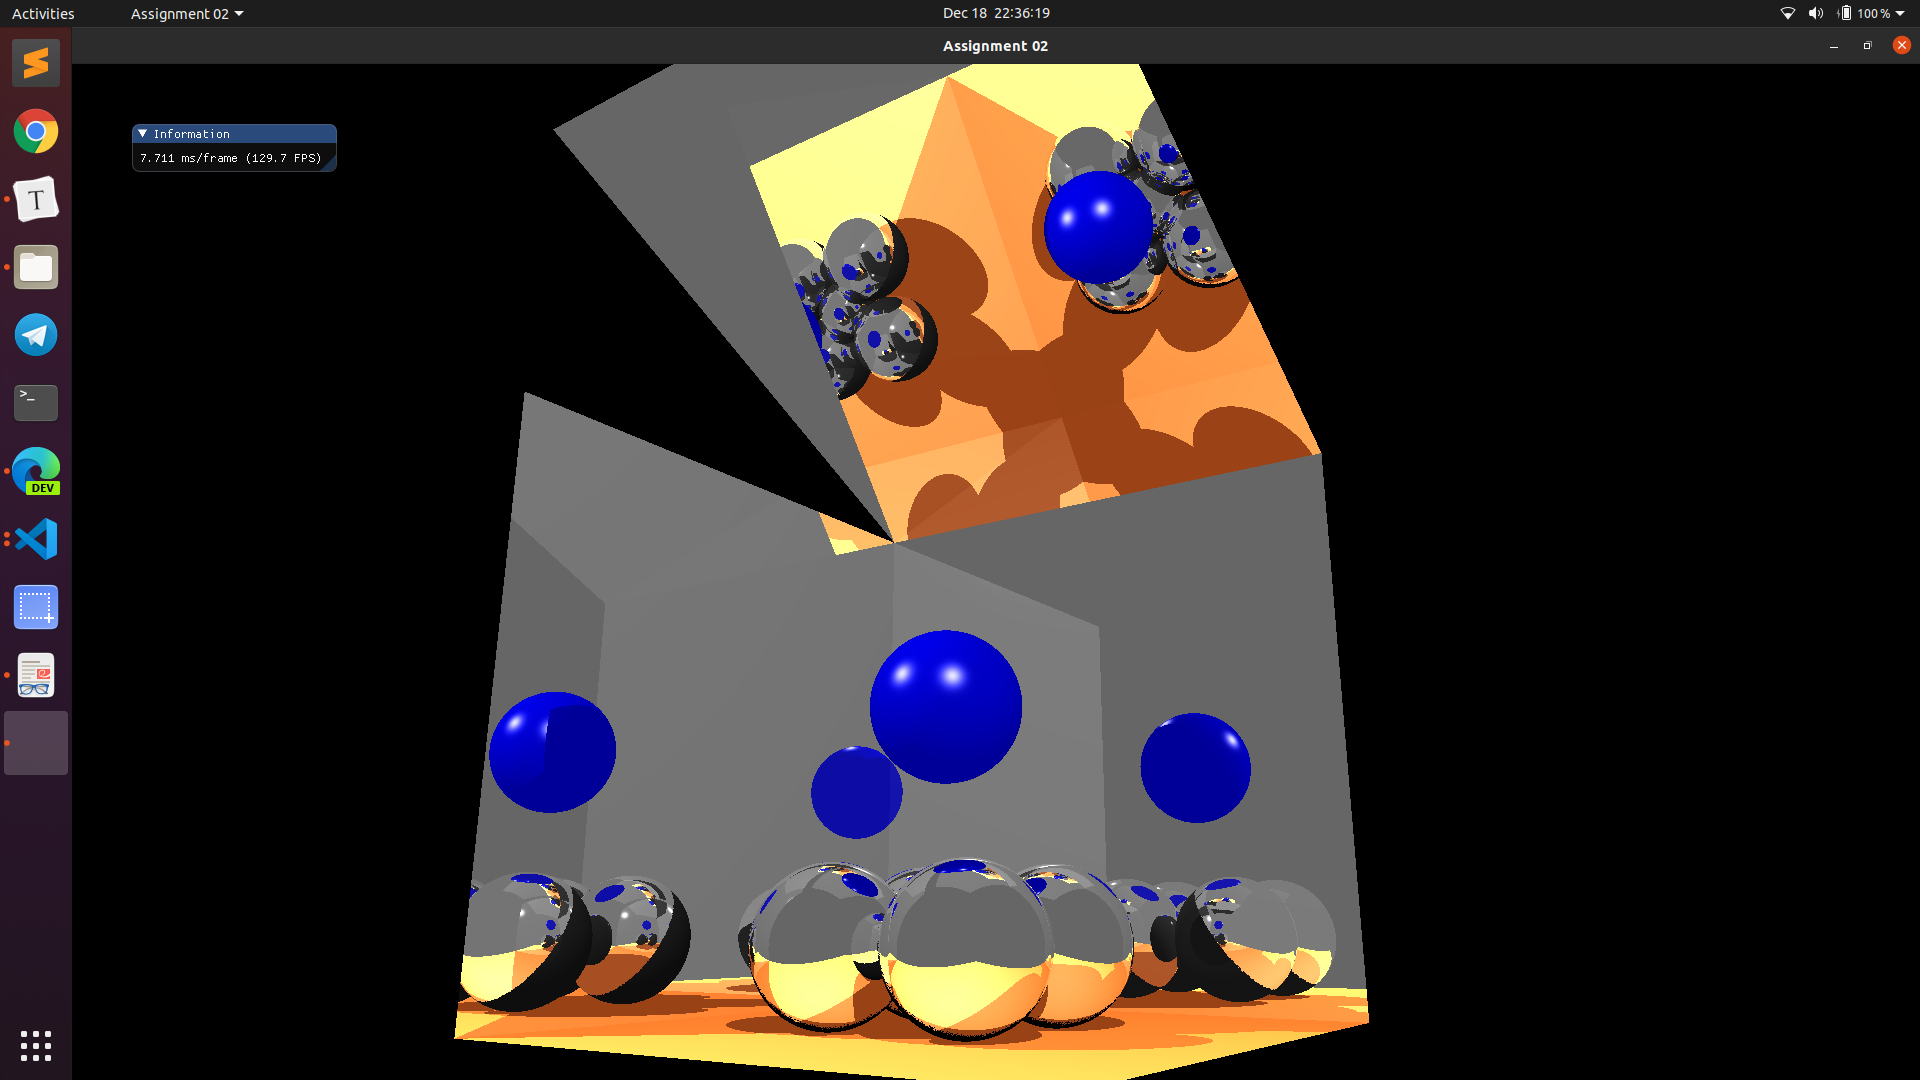
\includegraphics[width=0.8\textwidth]{Images/PanoramicView.png}
    \caption{Panoramic View of the scene.}
\end{figure}

\bigskip

\section{Contributions}
\begin{itemize}
    \item Project Setup : Aditya and Gaurav 
    \item Camera : Aditya
    \item Ray-Object Intersections : Aditya and Gaurav
    \item Blinn-Phong Shading : Aditya 
    \item Reflection : Aditya
    \item Presentation and Report: Gaurav 
\end{itemize}

Research :
\begin{itemize}
    \item Aditya $50\%$
    \item Gaurav $50\%$
\end{itemize} 
\vspace{\baselineskip}
Implementation : 
\begin{itemize}
    \item Aditya $70\%$
    \item Gaurav $30\%$
\end{itemize}
\vspace{\baselineskip}
Presentation and Report :
\begin{itemize}
    \item Aditya $30\%$
    \item Gaurav $70\%$
\end{itemize}

\bigskip

\printbibliography
\end{document}
